\documentclass{article} 
% \usepackage{iclr2026_conference,times}
\usepackage{macros}
\usepackage{natbib}
\usepackage{url}
\usepackage[toc,page,header]{appendix}
\usepackage{geometry}
\geometry{margin=1in}

\usepackage{minitoc}

\renewcommand \thepart{}
\renewcommand \partname{}

\title{Spectral State Space Models for Horizontal Connections and Video Modeling}

\author{}

\newcommand{\greg}[1]{\par\noindent{\color{indigo}[Gregoire]: #1}\par}
\newcommand{\TS}[1]{\par\noindent{\color{red}[TS]: #1}\par}

\begin{document}

\doparttoc % Tell to minitoc to generate a toc for the parts
\faketableofcontents % Run a fake tableofcontents command for the partocs

\maketitle

\begin{abstract}
...
\end{abstract}

\section{Introduction}


\paragraph{}Visual perception relies on the integration of information across space and time. In the visual cortex, neurons are organized topographically and interact through local horizontal connections, allowing activity to propagate across the visual field while preserving structure. These circuits are thought to underlie key perceptual phenomena such as contour integration and perceptual grouping, where global structure emerges from repeated local interactions.

\paragraph{}Computational models have long sought to capture this principle. Architectures based on horizontal recurrent interactions implement local connectivity together with iterative processing, enabling the emergence of long-range dependencies from short-range computations. However, these models are typically formulated as nonlinear recurrent neural networks (RNN), which are inherently sequential and therefore difficult to scale to large inputs or long time horizons. As a result, there is a gap between biologically grounded models of horizontal processing and modern scalable architectures.

\paragraph{}State space models (SSMs) have recently emerged as a powerful alternative for sequence modeling, combining linear recurrent dynamics with efficient parallel algorithms. Their favorable scaling properties make them an appealing backbone for modeling long-range dependencies. This raises a natural question: can SSMs serve as a scalable foundation for models of horizontal interactions? Existing extensions of SSMs to high-dimensional data suggest a negative answer. Current approaches either decouple spatial and temporal dynamics or restrict spatial interactions in a way that eliminates true spatio-temporal coupling. More fundamentally, directly incorporating convolutional spatial interactions into SSMs leads to a kernel growth phenomenon that breaks the parallel algorithms underlying their efficiency.

\paragraph{}In this work, we resolve this limitation by introducing a spectral formulation of convolutional state space models. By exploiting the fact that convolutional operators are diagonalized in the Fourier domain, we transform \emph{spatio-temporal entanglement} into \emph{decoupled frequency channels}. This representation preserves both spatio-temporal interactions and efficient parallel computation.

We introduce the Spectral Convolutional State Space Model (ConvSSM), a scalable framework that combines the inductive bias of horizontal connectivity with the computational advantages of state space models. This formulation provides a principled backbone for computational models of visual processing, enabling the study of horizontal interactions in regimes that were previously inaccessible to recurrent approaches.

\section{The Spectral ConvSSM}

\paragraph{The SSM.} is a class of recurrent model with linear recurrent dynamics. Their most general formulation is that of continuous-time (\Cref{eq:ssm}), which can be discretised as in \Cref{eq:ssm:recurrence}, with transition matrices depending on the desired step size following \Cref{eq:zoh}. This continuous time formulation allows the handling of arbitrary sampling rates for free.

\begin{minipage}[t]{.45\linewidth}
  \begin{subequations}
    \label{eq:ssm}
    \begin{align}
      \hvec'(t) &= \Amat \hvec(t) + \Bmat \xvec(t) \\
      \yvec(t) &= \Cmat \hvec(t) + \Dmat \xvec(t)
    \end{align}
  \end{subequations}
\end{minipage}%
\begin{minipage}[t]{.45\linewidth}
  \begin{subequations}
    \label{eq:ssm:recurrence}
    \begin{align}
    \label{eq:ssm:recurrence:1}
      \hvec_{t} &= \overline{\Amat} \hvec_{t-1} + \overline{\Bmat} \xvec_t \\
    \label{eq:ssm:recurrence:2}
      \yvec_t &= \Cmat \hvec_t + \Dmat \xvec_t
    \end{align}
  \end{subequations}
\end{minipage}%

\paragraph{Discretization.}
With zero-order hold (ZOH) and step size $\Delta$,
\begin{equation}
\label{eq:zoh}
\overline{\Amat} = e^{\Delta \Amat}
\qquad
\overline{\Bmat} = (\Delta \Amat)^{-1} (e^{\Delta \Amat} - \Imat) \cdot \Delta \Bmat .
\end{equation}

\begin{proposition}[SSM Complexity]
\label{prop:SSM_complexity}
    The parallel scan over the SSM has work and time complexity of:
\[
    W(\mathrm{Scan}) = O(T), \qquad T_\infty(\mathrm{Scan}) = O(\log T)
\]
\end{proposition}

\paragraph{Diagonal SSMs.} In the case of scalar inputs and the convolutional representation, \citet{gu2022s4d} show that if the transition matrix $\Amat$ is well conditioned, computing the convolution kernel only requires knowing its spectrum $\sigma(\Amat)$. For any vector-valued input SSM, with $\Amat = \Pmat \Lmat \Pmat^{-1}$ diagonalizable, we can rewrite the SSM as follows:
%
\begin{align}
\label{eq:ssm:diagonal}
\widetilde{\Amat} = \Lmat \qquad \widetilde{\Bmat} = \Pmat^{-1} \Bmat \qquad \widetilde{\Cmat} = \Cmat \Pmat
\end{align}
These two formulations are equivalent in the sense that they produce the same output $\widetilde{\yvec}(t)=\yvec(t)$, with hidden states linearly related by $\widetilde{\hvec}(t) = \Pmat^{-1} \hvec(t)$. The diagonal formulation allows to reduce the constant factors in \Cref{prop:SSM_complexity} from $O(N^3)$ to $O(N)$, as shown in \cref{app:constant_factors}.

% \TS{$O(N)$ always true here, or only under extra assumptions?}

\section{Convolutional State Space Models}

\subsection{The ConvSSM}
\label{sec:horizontal_connections}
% \TS{\textbf{CUT}: the neuroscience motivation here (retinotopy, horizontal connections) is already in the intro. Don't repeat it. Start directly with the technical point: we want spatial coupling in the SSM, convolutions give us structured $A$, but this creates Challenge A + B. One short paragraph, no biology.}

% \paragraph{Computational Motivation.} Many high-dimensional signals, such as images or videos, exhibit strong local spatiotemporal structures. In the context of biological vision, neurons exploit this structure through (\emph{i}) spatial organization, with neurons arranged in a topographic manner that preserves spatial relationships—a property known as retinotopy \citep{TODO}—coupled with (\emph{ii}) local interactions, with neurons primarily connecting to their immediate neighbors in the visual cortex. These local interactions, often referred to as \emph{horizontal connections}, enable information to propagate across space and time while preserving natural structures such as locality.

% \paragraph{Algorithmic Motivation.} 
% Incorporating spatial dependencies into state space models allows the hidden state to evolve spatio-temporally, enabling the modeling of long-range spatial dependencies through repeated local interactions. This is key for biological plausibility, strong inductive biases, and algorithmic efficiency.
% %
% Indeed, introducing spatial interactions in high-dimensional settings comes with significant computational challenges. For inputs of size $h \!\times\! w \!\times\! c$, the state dimension scales as $N \sim 10^6$. Naively parameterizing dense interaction matrices $\Amat \in \R^{N \times N}$ is therefore intractable, both in terms of work and memory.
% %
% This necessitates the use of structured operators that reduce complexity while preserving expressivity. In particular, structured matrices admitting fast matrix-vector products are essential to leverage parallel algorithms such as the scan, and to ensure scalability to realistic data regimes.

\paragraph{} 
Our goal is to extend state space models to high-dimensional spatio-temporal data such as images and videos. This requires combining \emph{local interactions in space} with \emph{efficient long-range integrations in time}. Convolutions provide a natural inductive bias for spatial locality, while SSMs offer scalable temporal dynamics through linear recurrences. We therefore introduce convolutional state space models (ConvSSMs) as a principled translation of horizontal recurrent circuits into the SSM framework, unifying spatial coupling and temporal dynamics in a single, scalable model.
%
Rewriting the SSM equations (\Cref{eq:ssm}) for kernel convolutions, we get the following spatial ConvSSM:

\begin{minipage}[t]{.45\linewidth}
\vspace{-5mm}
  \begin{subequations}
    \label{eq:conv_ssm_continuous}
    \begin{align}
    \label{eq:conv_ssm_continuous:1}
      \frac{\partial \hvec}{\partial t}(r,t) &= \Kmat_h \ast \hvec(r, t) + \Kmat_x \ast \xvec(r, t) \\
      \yvec(r, t) &= \Kmat_y \ast \hvec(r, t)
    \end{align}
  \end{subequations}
\vspace{-5mm}
\end{minipage}%
\begin{minipage}[t]{.45\linewidth}
\vspace{-5mm}
  \begin{subequations}
    \label{eq:conv_ssm_discrete}
    \begin{align}
    \label{eq:conv_ssm_discrete:1}
      \hvec_{t} &= \overline{\Kmat}_h \ast \hvec_{t-1} + \overline{\Kmat}_x \ast \xvec_t \\
    \label{eq:conv_ssm_discrete:2}
      \yvec_t &= \Kmat_y \ast \hvec_t
    \end{align}
  \end{subequations}
\vspace{-5mm}
\end{minipage}

Where $r$ is the spatial position, $\Kmat$ are convolution kernels and $\ast$ is the convolution operator. However, the spatial ConvSSM faces two closely linked challenges as a direct consequence of spatio-temporal coupling.
%
(\emph{Challenge A:}) Left in this format, it is not clear how to compute discrete-time kernels $\overline{\Kmat}_h$ and $\overline{\Kmat}_x$ from their continuous-time counterparts $\Kmat_h$ and $\Kmat_x$, or what such kernels would even look like. Specifically, \Cref{eq:zoh} requires matrices and cannot be applied to get the discrete-time kernels $\overline{\Kmat}_h$ and $\overline{\Kmat}_x$.
%
(\emph{Challenge B:}) parallel algorithms break down when adapted to the spatial ConvSSM (\Cref{prop:Spatial_ConvSSM_complexity}).

\begin{proposition}[Spatial ConvSSM Complexity]
\label{prop:Spatial_ConvSSM_complexity}
    Let $(\mathcal{M}, \oplus, e)$ be the monoid corresponding to the spatial convolutional SSM, defined by \Cref{eq:M_SSM,eq:+_SSM,eq:0_SSM}. Let $(a_i)_{i\in \intint{0}{T-1}}\in \mathcal{M}^{\intint{0}{T-1}}$. Then, the parallel scan over $(a_i)$ has work and time complexity of:
\[
    W(\mathrm{Scan}) = T_\infty(\mathrm{Scan}) = O(T^2)
\]
\end{proposition}

\begin{proof}
See \cref{app:Spatial_ConvSSM_complexity}. Key observation: $\oplus$ uses the block convolution operator $\circledast$, which produces kernels of size \textbf{exponential in depth}. Therefore, the scan is no longer $O(1)$ per $\oplus$ operation.
\end{proof}

% \TS{\textbf{KEY TRANSITION}: after restructuring, this is where the spectral SSM material (currently in its own section) lands. The ``introduced in the previous section'' reference goes away -- instead you INTRODUCE the Fourier diagonalization here as the solution to the challenges stated above. Bring in the BCCB $\to$ Fourier material, then apply it to the ConvSSM. One fluid derivation instead of two disconnected ones.}

\subsection{Spectral ConvSSMs}

\paragraph{} These are not implementation issues but structural. To circumvent both challenges, we move from a spatial to a spectral representation of the ConvSSM. Spectral representations offer the natural basis we need by decomposing spatio-temporal entanglement into independent frequency channels. We start by stacking all spatial positions and channels into a single vector, and rewrite the convolutions as matrix-vector products.
%
Indeed, discrete-space convolutions correspond to linear operators with a block-circulant with circulant blocks (BCCB) structure (\Cref{eq:convssm:spatial}), leading to an SSM with $d = h w c_\mathrm{in}$-dimensional inputs and outputs, and $N = h w c$-dimensional hidden states:
%
\begin{align}
\label{eq:convssm:spatial}
\Amat = \mathrm{Circ}(\Kmat_h) \qquad \Bmat = \mathrm{Circ}(\Kmat_x) \qquad \Cmat = \mathrm{Circ}(\Kmat_y)
\end{align}
%
These matrices are diagonalized by the Fourier transform. We can thus introduce the \emph{Spectral State Space Model}.

\paragraph{Spectral State Space Models.} Consider the case where $\Amat$ is block-circulant with blocks of size $c \!\times\! c$. This can be rewritten as a 1D convolution over $\frac{N}{c}$ positions and $c$ channels. Let $\Fmat_{\frac{N}{c}} \in \R^{\frac{N}{c} \times \frac{N}{c}}$ be the Fourier matrix. Then, $\Amat$ is diagonalized by $\Pmat = \Fmat \otimes \Imat_c$, where $\otimes$ is the Kronecker product. It can be written as $\Amat = (\Fmat \otimes \Imat_c) \Lmat_c (\Fmat^{-1} \otimes \Imat_c)$, where $\Lmat_c$ is a block-diagonal matrix with blocks of size $c \!\times\! c$. The resulting SSM is what we call a Spectral State Space Model (SSSM).

The core idea of SSSMs is to constrain $\Amat$ not only such that it is structured after some change of basis $\Pmat$, but such that $\Pmat$ itself is structured, allowing for efficient matrix-matrix and matrix-vector products. This isn't restricted to 1D fourier transforms. For example, this still works when $\Fmat_{\frac{N}{c}}$ is replaced by $\Fmat_h \otimes \Fmat_w$ for 2D convolutions.
%
\begin{align}
\label{eq:ssm:spectral}
\widetilde{\Amat} = \Lmat_c \qquad \widetilde{\Bmat} = \Pmat^{-1} \Bmat \qquad \widetilde{\Cmat} = \Cmat \Pmat
\end{align}

\paragraph{Diagonal SSSMs.} At this point, we have \Cref{eq:ssm:spectral} where the change of basis is structured. This means that powering $\widetilde{\Amat}$ costs $O(\frac{N}{c} c^3) = O(N c^2)$. We go back to the diagonal case where powering $\Amat$ only costs $O(N)$, as this is the bottleneck in parallel algorithms (\cref{app:constant_factors}). We can write $\widetilde{\Amat} = \Qmat_c \Lmat \Qmat_c^{-1}$, where $\Lmat$ is diagonal and $\Qmat_c$ is a block-diagonal matrix with blocks of size $c \!\times\! c$. Essentially, $\Qmat_c$ captures channel mixing withing each frequency block in $\Lmat_c$, and leaves a pure diagonal $\Lmat$. We get the following diagonal SSM:
%
\begin{align}
\label{eq:ssm:diagonal_spectral}
\widehat{\Amat} = \Lmat \qquad \widehat{\Bmat} = \Qmat_c^{-1} \Pmat^{-1} \Bmat \qquad \widehat{\Cmat} = \Cmat \Pmat \Qmat_c
\end{align}

\paragraph{The Spectral ConvSSM.} In order to combine \Cref{eq:convssm:spatial,eq:ssm:diagonal_spectral} we proceed to the following reformulation. \textbf{(A)}~First, we move from convolution operators to their BCCB matrix counterpart. \textbf{(B)}~Then, we diagonalize these BCCB matrices through the Fourier transform. We are left with block-diagonals instead of pure diagonals due to channel mixing. \textbf{(C)}~The final step is therefore to absorb the channel mixing of the recurrent dynamics into the input and output transforms $\Bmat$ and $\Cmat$. We begin by can rewrite the convolutional SSM as:
%
\begin{align}
\label{eq:convssm:A}
\Amat &= \mathrm{Circ}(\Kmat_h) = \Pmat \Lmat^A_c \Pmat^{-1} = \Pmat \Qmat_c \Lmat \Qmat_c^{-1} \Pmat^{-1} \\
\label{eq:convssm:B}
\Bmat &= \mathrm{Circ}(\Kmat_x) = \Pmat \Lmat^B_c \Pmat_{\mathrm{in}}^{-1} \\
\label{eq:convssm:C}
\Cmat &= \mathrm{Circ}(\Kmat_y) = \Pmat_{\mathrm{in}} \Lmat^C_c \Pmat^{-1}
\end{align}
%
with $\Pmat = (\Fmat_h \otimes \Fmat_w) \otimes \Imat_c$, $\Pmat_{\mathrm{in}} = (\Fmat_h \otimes \Fmat_w) \otimes \Imat_{c_\mathrm{in}}$. $\mathrm{Circ}(\Kmat)$ is the convolution operator with kernel $\Kmat$, and the $\Lmat^{\cdot}_c$ are block-diagonal matrices with blocks of size $c \!\times\! c$, $c \!\times\! c_\mathrm{in}$ and $c_\mathrm{in} \!\times\! c$, respectively, corresponding to the Fourier transform of the convolution kernels.
%
This decomposition can therefore be written as a diagonal SSSM, where all the computational load is absorbed by $\Bmat$ and $\Cmat$:

\begin{align}
\label{eq:convssm}
&\boxed{\widehat{\Amat} = \Lmat} \\
&\widehat{\Bmat} = \Qmat_c^{-1} \Pmat^{-1} \Pmat \Lmat^B_c \Pmat_{\mathrm{in}}^{-1} = \left(\Qmat_c^{-1} \Lmat^B_c\right) \Pmat_{\mathrm{in}}^{-1} \boxed{= \Lmat^{B'}_c \Pmat_{\mathrm{in}}^{-1}} \\
&\widehat{\Cmat} = \Pmat_{\mathrm{in}} \Lmat^C_c \Pmat^{-1} \Pmat \Qmat_c = \Pmat_{\mathrm{in}} \left(\Lmat^C_c \Qmat_c\right) \boxed{= \Pmat_{\mathrm{in}} \Lmat^{C'}_c}
\end{align}

This formulation makes it apparent that the tension in \emph{Challenge A} is that the discretized kernels have full spatial support, rendering the spatial convolution representation inapplicable. The Spectral ConvSSM trivializes the discretization process through diagonalization, and bypasses prohibitive convolutions through efficient matrix multiplications.
%
Similarly, \emph{Challenge B} also boils down to kernel size explosion, and is bypassed by the spectral formulation for the same reason. We derive the full complexity analysis in \cref{app:complexity_proofs} and point exactly where the kernel explosion happens for the spatial ConvSSM, and how the spectral formulation avoids~it.

\begin{proposition}[Spectral ConvSSM Complexity]
\label{prop:Spectral_ConvSSM_complexity}
    Let $(\mathcal{M}, \oplus, e)$ be the monoid corresponding to the spectral convolutional SSM, defined by \Cref{eq:M_SSM,eq:+_SSM,eq:0_SSM}. Let $(a_i)_{i\in \intint{0}{T-1}}\in \mathcal{M}^{\intint{0}{T-1}}$. Then, the parallel scan over $(a_i)$ has work and time complexity of:
\[
    W(\mathrm{Scan}) = O(T), \qquad T_\infty(\mathrm{Scan}) = O(\log T)
\]
\end{proposition}

\begin{proof}
See \cref{app:Spectral_ConvSSM_complexity}. Key observation: the scan is $O(1)$ per $\oplus$ operation.
\end{proof}

\subsection{Link with previous work}

Previous approaches such as ConvS5 \citep{smith2023convs5} faced these challenges by forfeiting horizontal connections. They restrict the transition operator to act independently at each spatial location, typically using $1 \!\times\! 1$ convolutions in \Cref{eq:conv_ssm_continuous}. Equivalently, in the stacked vector representation (\Cref{eq:convssm:spatial}), this corresponds to replacing the circulant structure of $\Amat$ with a block diagonal with constant blocks $\Amat = \Imat_{hw} \otimes \Kmat$~-~where $\Kmat \in \R^{c \times c}$.

This constraint removes spatio-temporal coupling from the temporal ODE, i.e., the "Conv" in "ConvS5". In contrast, our approach explicitly models spatio-temporal coupling, disentangling it through the spectral domain while retaining the computational benefits of structured state space models.

\subsection{Final Model}
\label{sec:final_model}

\greg{Find a better section title...}

\paragraph{The Core.} \greg{Spectral ConvSSM}

\paragraph{Parameterization.} \greg{Rework this paragraph} We parameterize $\Amat$ as a complex-valued vector $\Lmat \in \C^N$. As for $\Bmat$ and $\Cmat$, we can either parameterize them as kernels in the spatial domain, or as block-diagonal matrices in the spectral domain.
%
The spatial parameterization leads to input and output transforms of $O(c c_\mathrm{in} k^2)$ parameters and either $\underbrace{O(hwk^2cc_\mathrm{in})}_{\text{spatial convolution}} + \underbrace{O(hw \log(hw) c)}_{\text{FFT}}$ or $\underbrace{O(hwcc_\mathrm{in})}_{\text{spectral product}} + \underbrace{O(hw \log(hw) c c_\mathrm{in})}_{\text{FFT}}$ complexities depending on the order of operations.
%
The spectral parameterization leads to $O(hwcc_\mathrm{in})$ parameters with complexity of $O(hwcc_\mathrm{in})$.

\paragraph{Stability.} \greg{eigenvalues of $A$}

\paragraph{Circuits.} \greg{All circuit derivation on the SSM applies to our core. We take Gated Delta Net as state of the art circuit and plug it on top of our core.}

\section{Scaling Laws}

\section{Benchmarks}

\section{Fine Tuning for Video Modeling}

\section{Interpretability}

\section{Related Work}

\paragraph{}State space models (SSMs) have recently emerged as a powerful alternative to attention-based architectures for long-range sequence modeling, combining linear recurrent dynamics with efficient parallel algorithms. Early work on structured state space models builds on the HiPPO framework~\citep{gu2020}, which introduced principled continuous-time representations of long-range dependencies, and culminates in S4~\citep{gu2022}, where carefully parameterized transition matrices together with a convolutional representation and parallel algorithms enable efficient modeling of long sequences. Subsequent work has further simplified and structured SSMs along multiple axes to improve efficiency and scalability. Diagonal parameterizations~\citep{gu2022s4d, gupta2022} reduce computational cost while retaining performance, while extensions from single-input single-output to multi-input multi-output~\citep{smith2023s5} formulations were enabled by efficient parallelization through scan algorithms.

Additional refinements such as linear recurrent units (LRUs)~\citep{orvieto2023} and gating mechanisms~\citep{mehta2023} further enhance expressivity and stability. Further circuit derivations and refinements around the core of SSMs include input-dependent selection of transition matrices in Mamba~\citep{gu2023}, and the SSM--attention duality in Mamba-2~\citep{dao2024} through the lens of semiseparable matrices. However, these advances remain fundamentally limited to one-dimensional sequence modeling and do not natively capture spatial structure.

\paragraph{}Extending SSMs to high-dimensional visual data such as images and videos requires incorporating dynamics over multiple axes. S4ND~\citep{nguyen2022} introduces precisely this extension, formalising SSMs evolving over multiple dimensions through separable dynamics. Though successful as a drop-in replacement for state-of-the-art visual processing layers, S4ND's fundamental separation between space and time limits its ability to capture spatio-temporal coupling. Other SSM-based approaches to vision and video modeling have emerged~\citep{zhu2024,li2024videomamba,li2024mamband}.

True spatio-temporal coupling was formulated in~\citet{smith2023convs5}. Their ConvS5 beats ConvLSTMs and Transformers on long-horizon video modeling. However, ConvS5's convolutional recurrence is limited to $1 \!\times\! 1$ kernels, thereby forfeiting spatio-temporal coupling of the ConvSSM. This is not a mere design choice, but a fundamental consequence of parallelising over coupled spatio-temporal dynamics. In contrast, our Spectral ConvSSM formulation explicitly models spatio-temporal coupling through the spectral domain while retaining the computational benefits of structured state space models.

\section{Conclusion}

\bibliography{references}
\bibliographystyle{plainnat}

\newpage
\appendix

\section{Complexity Proofs}
\label{app:complexity_proofs}

We analyse the complexity of the parallel scan algorithm to show why convolutions in spatial domain make the complexity explode, and how doing convolutions in spectral domain preserves $O(\log T)$ complexity. We consider both the work complexity $W$, measuring the total amount of atomic operations to perform, and the time complexity under unlimited parallelization $T_\infty$, measuring the longest sequence of atomic operations remaining after optimal parallelization.

We begin by addressing the main issue of the complexity explosion of convolutional SSMs in \cref{app:parallel_scan,app:SSM_complexity,app:Spatial_ConvSSM_complexity,app:Spectral_ConvSSM_complexity}. Our main result is \Cref{prop:Spectral_ConvSSM_complexity}. We show in \cref{app:Spectral_ConvSSM_complexity} that we can achieve the same work and time complexity as a regular linear SSM. We then tackle the question of reducing the constant to make it tractable, using standard tricks, adapted to our framework, in \cref{app:constant_factors}.

\subsection{The Parallel Scan}
\label{app:parallel_scan}

We first describe the parallel scan operation in the most general way. This operation is the core of the SSM parallelization. Let $(a_i)_{i\in I}\in \mathcal{M}^I$ be elements of a monoid $(\mathcal{M},\oplus,e)$, with $I=\intint{0}{T\!-\!1}$. The parallel scan is an algorithm that computes $(s_i=\sum_{j=0}^ia_j)_i\in I$. This algorithm is parallelisable and requires associativity of the $\oplus$ operator and a neutral element $e$, hence the minimal requirement of a monoid structure. It proceeds in two sweeps mirroring each other. The first sweep proceeds in a tree like structure, with level $l$ of the tree computing $a^{l+1}_{k}\coloneqq a^l_{2k} \oplus a^l_{2k+1}$, and initialised with $a^0_k\coloneqq a_k$. Once this upward sweep is over, the downward sweep computes mirror operations, with $b^0_1\coloneqq e$ and $(b^{l+1}_{2k}, b^{l+1}_{2k+1}) = (b^{l}_{k}, b^{l}_{k} \oplus a^{\log_2(T)-(l+1)}_{2k})$. The order is crucial here as $\oplus$ is not required to be commutative. It is only required to be associative. In our application for SSM, it is not be commutative. We denote the parallel scan procedure as $\mathrm{Scan}((a_i)_{i\in I})$ or $\mathrm{Scan}$ for short.
\Cref{fig:parallel_scan_general} provides a visualisation of the entire procedure.

\begin{figure}[ht]
    \centering
    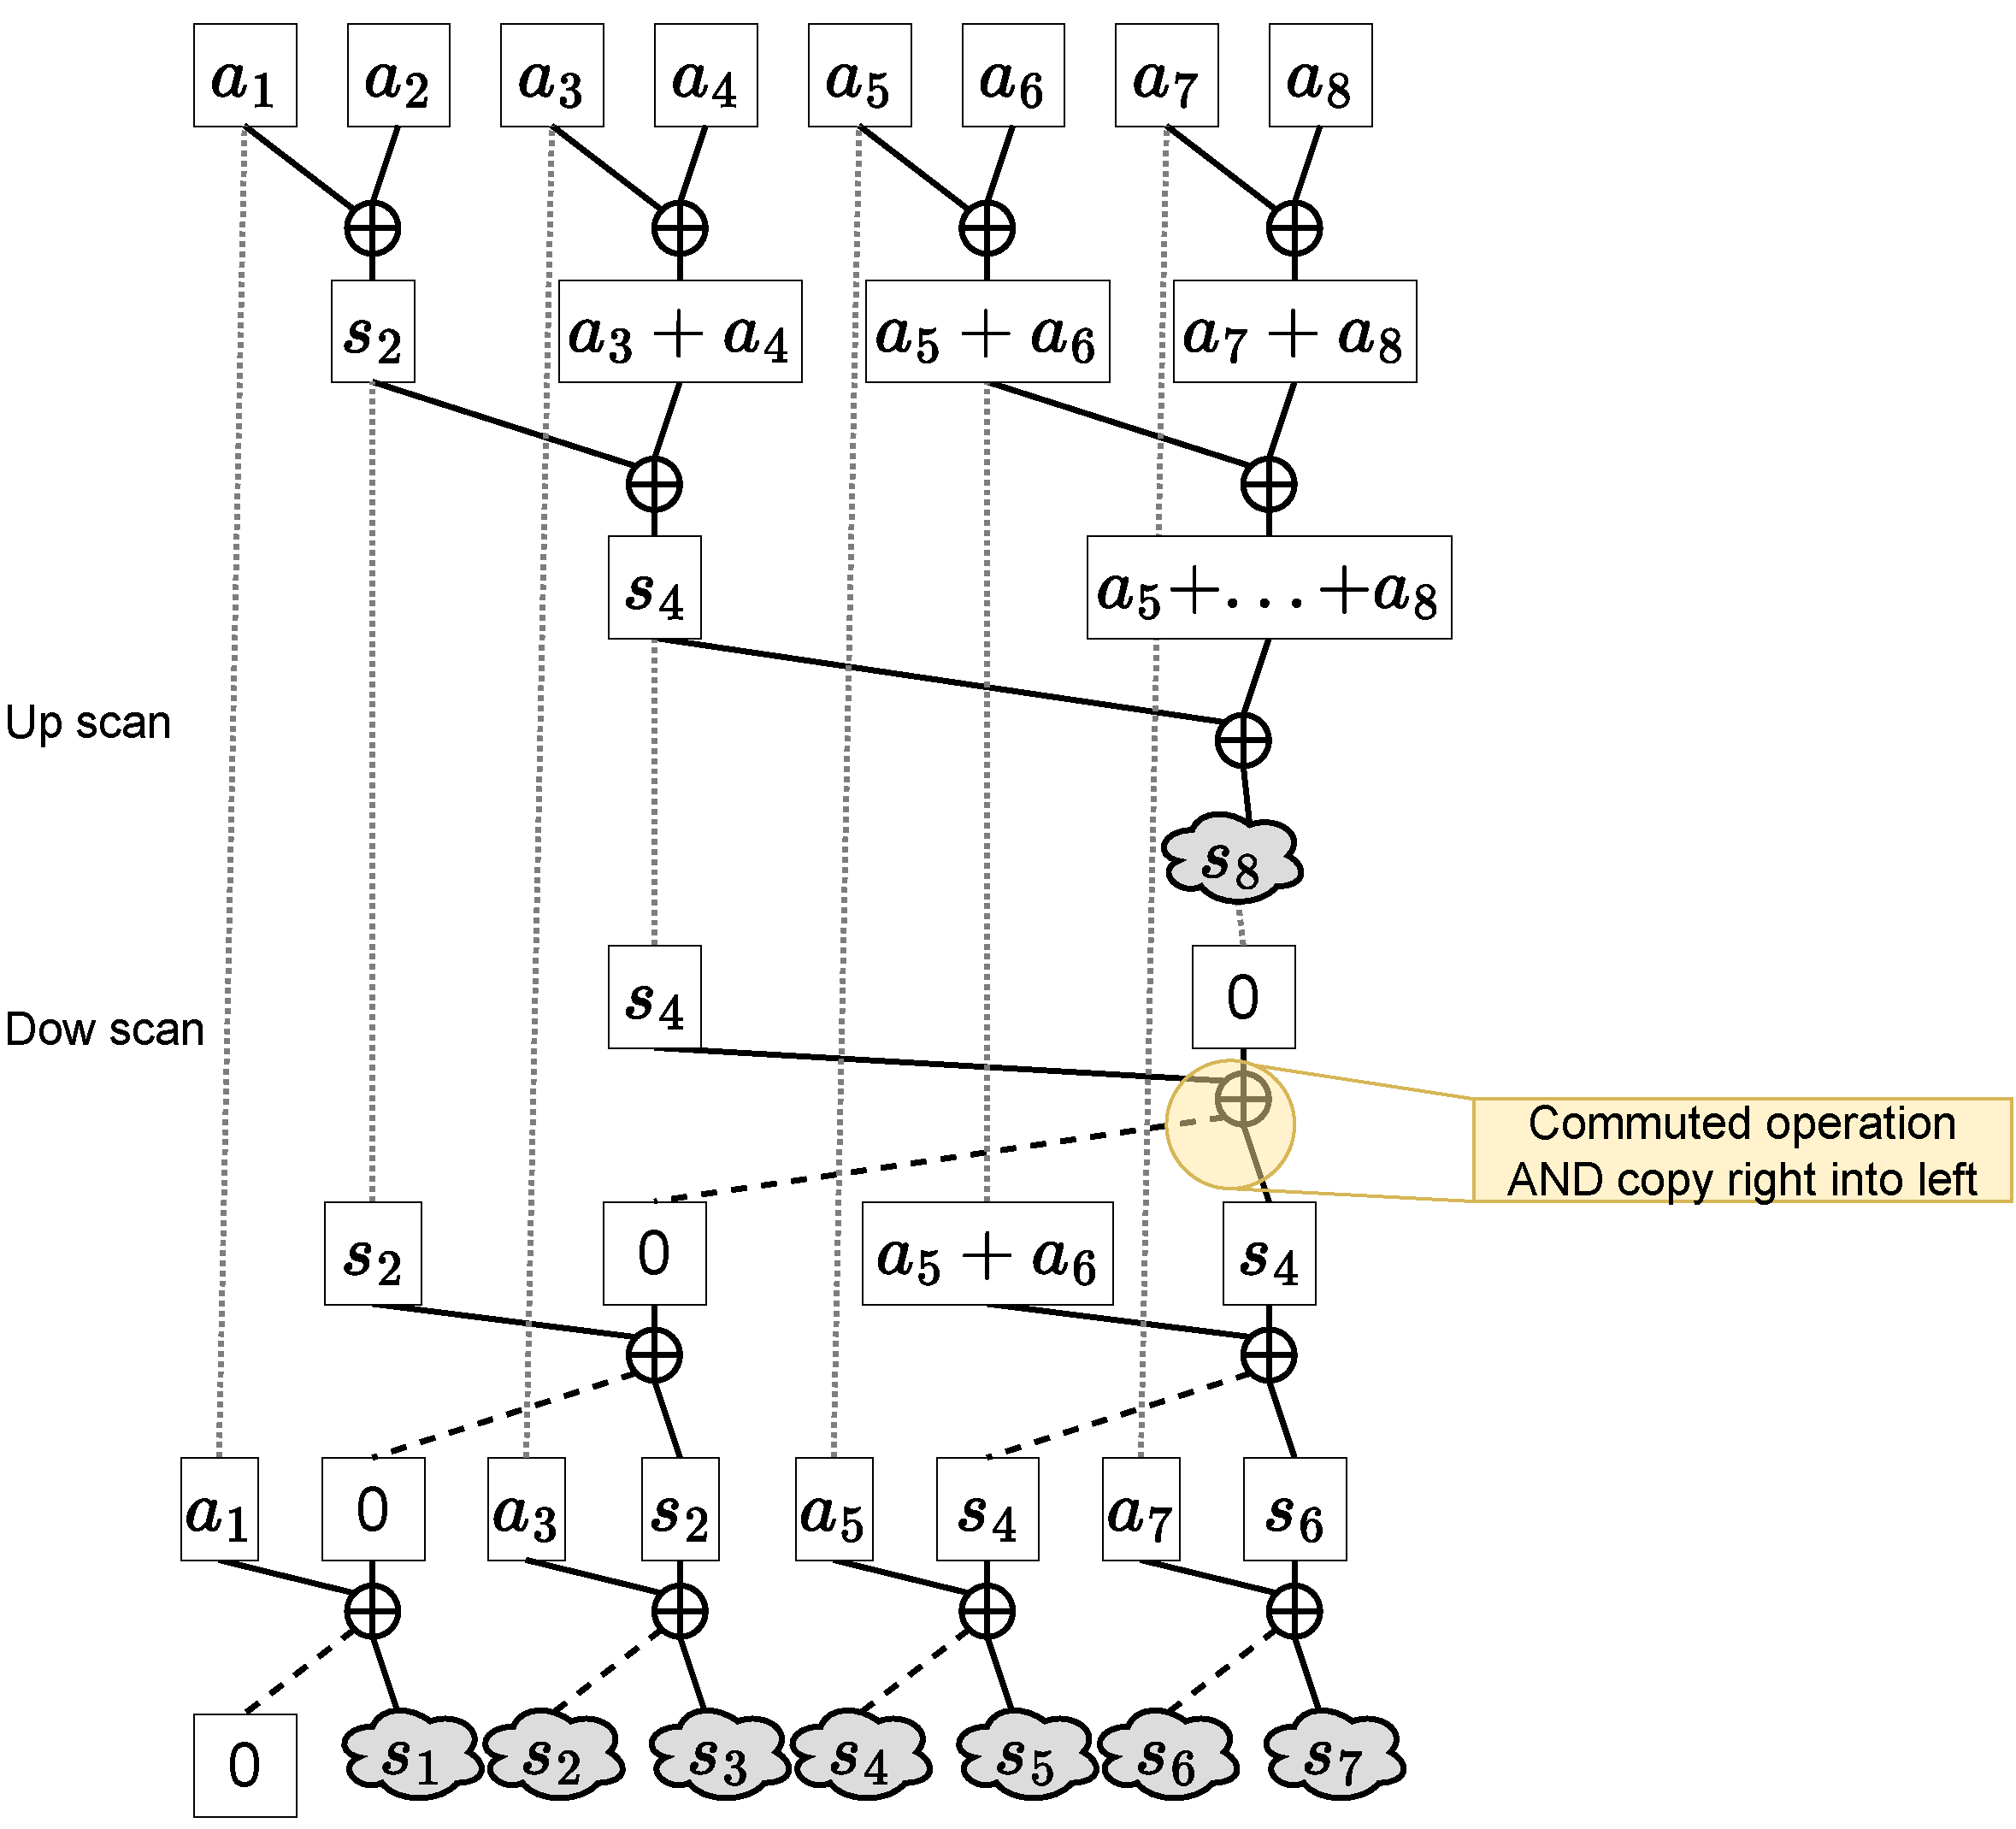
\includegraphics[height=0.3\textheight]{figures/scan_monoid.pdf}
    \hspace{20mm}
    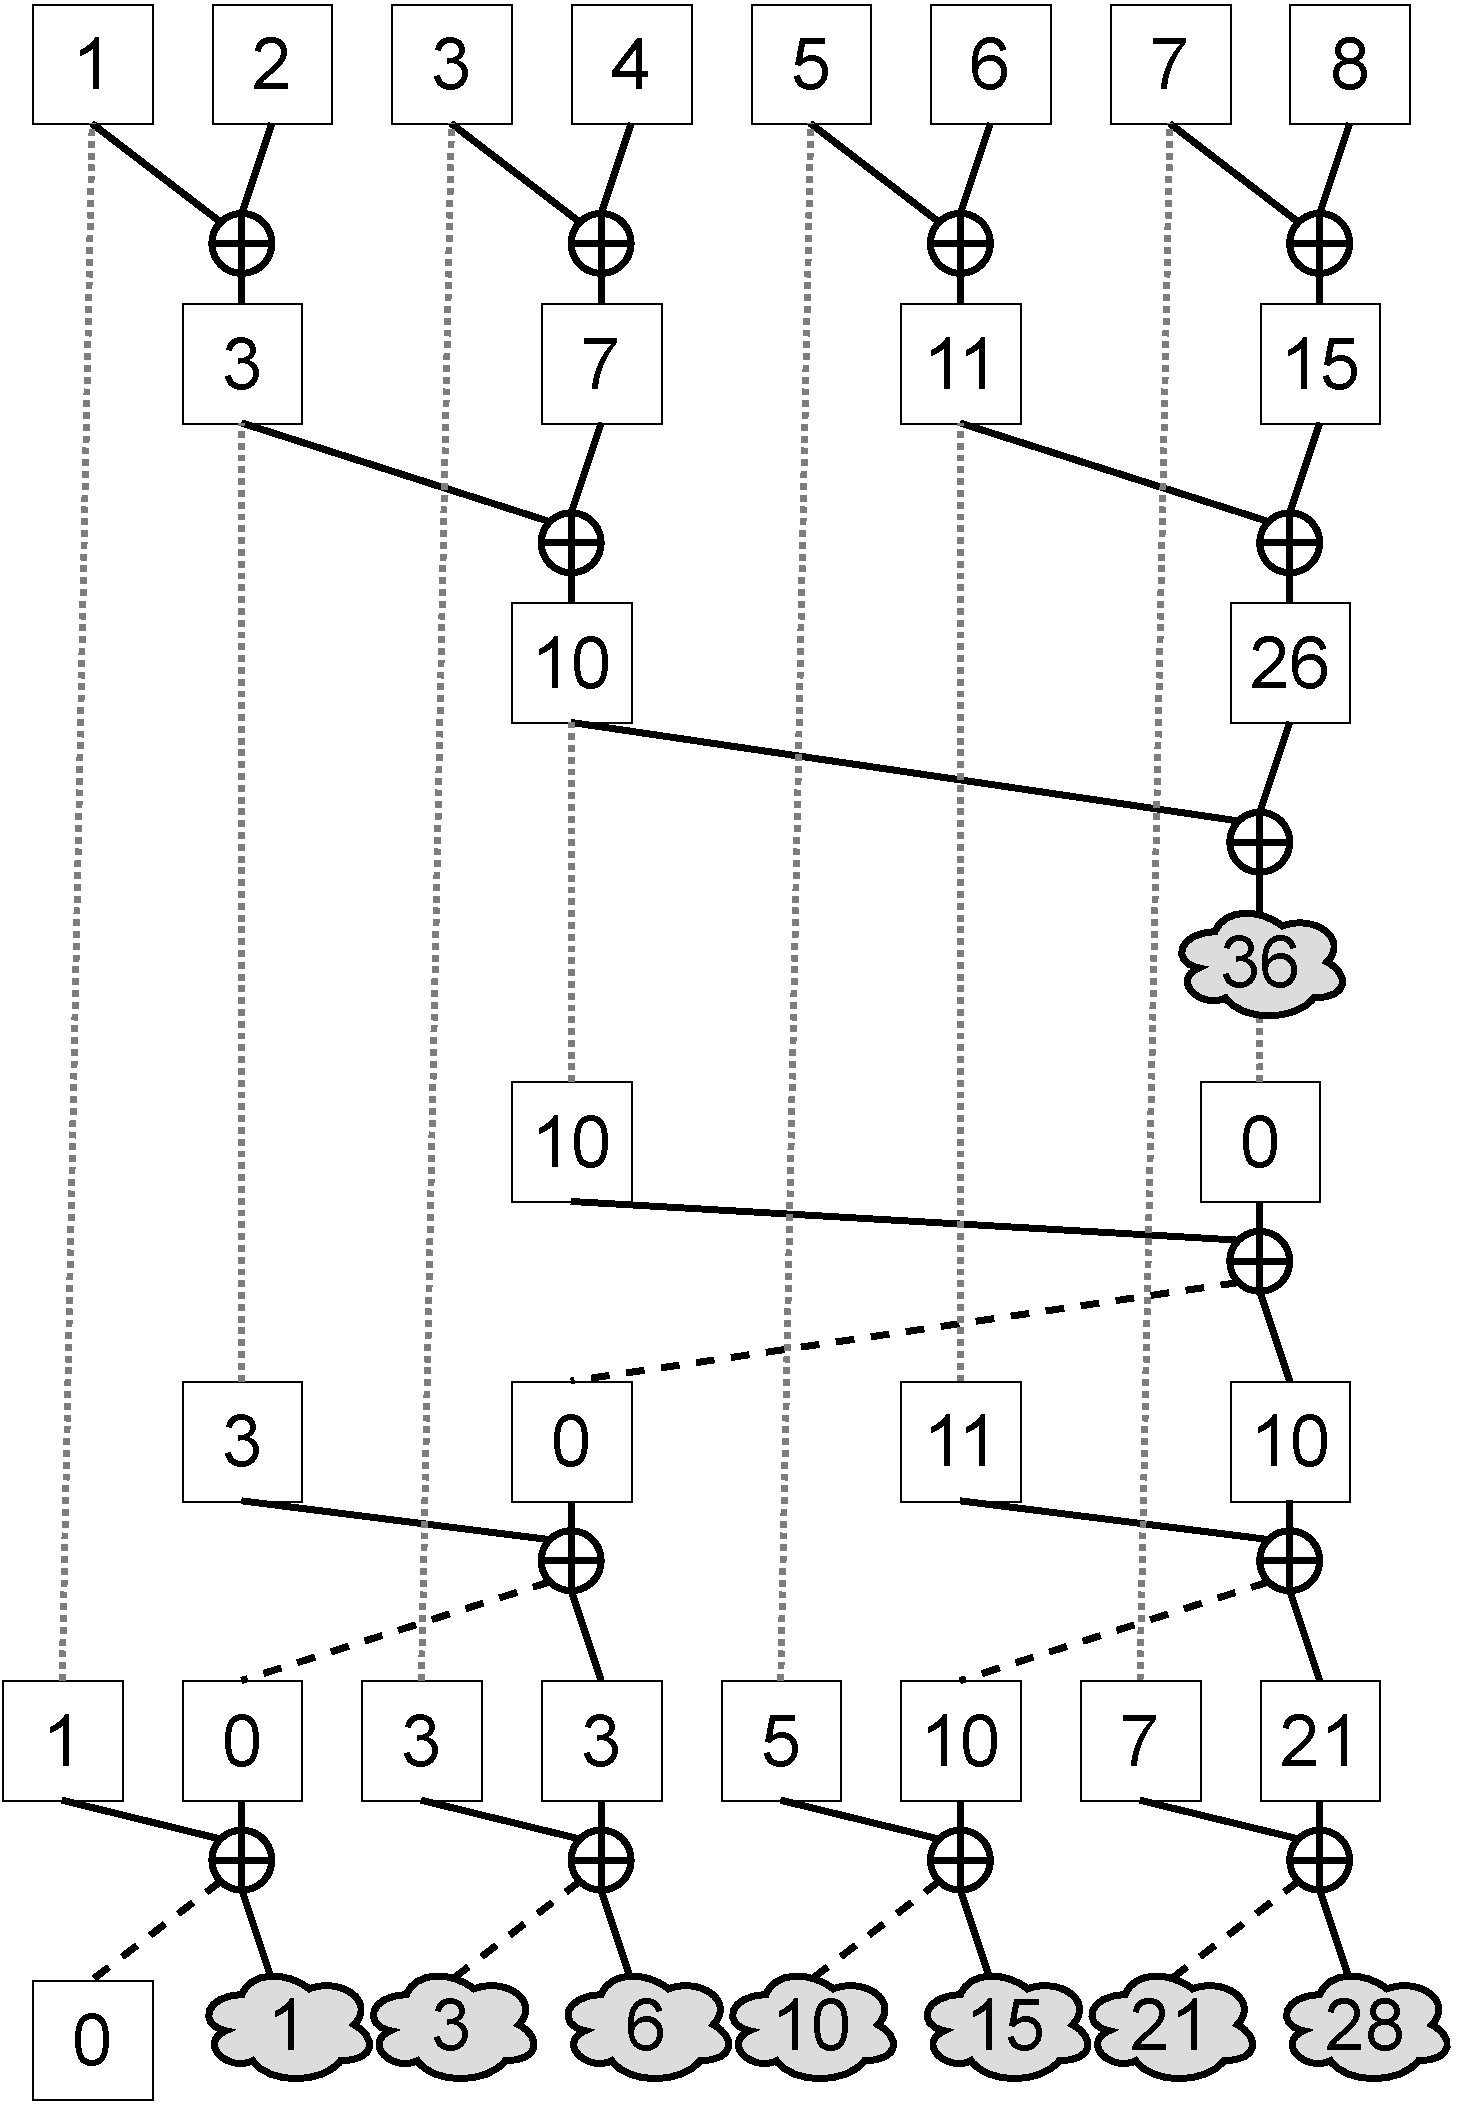
\includegraphics[height=0.3\textheight]{figures/scan_integer.pdf}
    \caption{\textbf{Left:} parallel scan with a generic monoid. \textbf{Right:} illustration on the special case of natural integers.}
    \label{fig:parallel_scan_general}
\end{figure}

The procedure described above yields $(\sum_{j=0}^{i-1}a_j)_{i\in I}$, with the cumulative sum being $a^{\log_2(T)}_{0}$ the intermediate result of the upward sweep. We analyse the work complexity $W$ and the time complexity $T_\infty$ of $\mathrm{Scan}$ in terms of floating point operations, where $W$ counts the total number of operations needed and $T_\infty$ counts the time complexity under unlimited parallelism.

\begin{proposition}[Parallel Scan Complexity for Integers]
\label{prop:scan_integer_complexity}
    Let $(\mathcal{M}, \oplus, e) \coloneqq (\N, +, 0)$ be the monoid of natural integers equipped with addition. Let $(a_i)_{i\in I}\in \N^I$ be a sequence of integers.

\begin{align}
    W(\mathrm{Scan})&= 2(T-1)\\
    T_\infty(\mathrm{Scan})&= 2\log_2 T
\end{align}
\end{proposition}

\begin{proof}
At level $l$ of the upward scan, $U_l = T/(2^{l+1})$ $\oplus$ operations are performed, each of them having a complexity of $1$. There are $\log_2 T$ levels in total. The same goes on for the downward scan, with $D_l = T/(2^{\log_2(T) - l})=2^{l}$ operations at level $l$. Therefore, the work complexity of level $l$ is $U_l$ (resp. $D_l$) while its time complexity is $1$ with unlimited parallelism. It follows that

\begin{align}
\label{eq:W_integer}
W &= 2\sum_{l=0}^{\log_2 T-1}2^l=2(T-1)\\
\label{eq:T_integer}
T_\infty&= 2\sum_{l=0}^{\log_2 T-1}1=2\log_2T
\end{align}
\end{proof}

The key point of this analysis is that the $\oplus$ operation has constant time complexity.

\subsection{SSM Complexity}
\label{app:SSM_complexity}

The case of SSMs is a little more complicated than that of real numbers. In SSMs, the recurrence is defined by \Cref{eq:ssm:recurrence}. We take $B = I$ and $d = N$ for simplicity. Thus, the goal is to compute in parallel the hidden states $(h_i = \sum_{j=0}^i\overline{A}^{i-j}x_j)_i\in I$, where $x_i$ are vectors of dimension $d$ and $\overline{A}$ is a square matrix. This is almost but not quite what we need for the parallel scan. We define the following monoid:
\begin{align}
\label{eq:M_SSM}
    &\mathcal{M}^{\mathrm{SSM}}\coloneqq \left\{a = (A, x)\mid A\!\in\!\mathcal{M}_{d}(\R),~x\!\in\!\R^d\right\}\\
\label{eq:+_SSM}
    &(A_a, x_a) \oplus^{\mathrm{SSM}} (A_b,x_b)\coloneqq (A_b \odot A_a, A_b \cdot x_a + x_b)\\
\label{eq:0_SSM}
    &e^{\mathrm{SSM}}\coloneqq(I_d, 0)
\end{align}

With this monoid structure, and the sequence $(a_t)_{t\in I} \coloneqq ((\overline{A}_t, x_t))_{t\in I} \in \mathcal{M}^I$, the result of the parallel scan is $((A^t, \sum_{j=0}^tA^{t-j}x_j))_{t\in I}$. The complexity of the scan is less straightforward, but the complexity of each $\oplus^{\mathrm{SSM}}$ operation depends only on $d$. It is a constant of $T$. Therefore, the overall time complexity of the scan is $T_\infty= O(\log T)$ and $W=O(T)$.

\begin{proposition}[SSM Complexity]
    Let $(\mathcal{M}, \oplus) \coloneqq (\mathcal{M}^{\mathrm{SSM}}, \oplus^{\mathrm{SSM}})$ be the monoid defined by \Cref{eq:M_SSM,eq:+_SSM,eq:0_SSM}. Let $(a_i)_{i\in I}\in (\mathcal{M}^{\mathrm{SSM}})^I$.

\begin{align}
    W(\mathrm{Scan})&= 2(T-1)(d^3+d^2+d)\\
    T_\infty(\mathrm{Scan})&= 2\log_2 (T) (d^3+d^2+d)
\end{align}
\end{proposition}

\begin{proof}
The proof of \Cref{prop:scan_integer_complexity} applies with the only difference that now, each $\oplus^{\mathrm{SSM}}$ operation has complexity $d^3$ for the matrix multiplication on the left, $d^2$ for the matrix-vector multiplication and $d$ for the vector addition on the right.
\end{proof}

\subsection{Spatial ConvSSM Complexity}
\label{app:Spatial_ConvSSM_complexity}

Rewriting the SSM (\Cref{eq:ssm:recurrence}) to the ConvSSM formulation of \Cref{eq:conv_ssm_discrete}, we can similarly adapt the monoid structure as :
\begin{align}
    &\mathcal{M}^{\mathrm{Conv}_1}\coloneqq \left\{a = (\Kmat, x)\mid \exists k_1, k_2,\quad \Kmat\!\in\!\R^{k_1\times k_2\times c\times c},~x\!\in\!\R^{h \times w \times c}\right\}\\
    &(\Kmat_a, x_a) \oplus^{\mathrm{Conv}_1} (\Kmat_b,x_b)\coloneqq (\Kmat_b \circledast \Kmat_a, \Kmat_b \ast x_a + x_b)\\
    &e^{\mathrm{Conv}_1}\coloneqq(I, 0)
\end{align}
\noindent where $\circledast$ is the block convolution between two kernels and $\ast$ is the convolution between a kernel and an image:

\begin{align*}
    & \forall \left\{
\begin{aligned}
    &i\!\in\!\intint{0}{h\!-\!1}\\
    &j\!\in\!\intint{0}{w\!-\!1}\\
    &c_{\mathrm{out}}\!\in\!\intint{1}{c}
\end{aligned}
\right., (\Kmat\!\ast\!x)_{i,j,c_{\mathrm{out}}} = \sum_{u=0}^{k_1-1}\sum_{v=0}^{k_2-1}\sum_{c_{\mathrm{in}}=1}^{c} \Kmat_{u,v,c_{\mathrm{in}},c_{\mathrm{out}}} x_{(i-u,j-v)\%(h,w),c_{\mathrm{in}}}\\
    & \forall \left\{
\begin{aligned}
    &u\!\in\!\intint{0}{k_1\!+\!l_1\!-\!2}\\
    &v\!\in\!\intint{0}{k_2\!+\!l_2\!-\!2}\\
    &c_{\mathrm{in}},c_{\mathrm{out}}\!\in\!\intint{1}{c}
\end{aligned}
\right., (L \circledast \Kmat)_{u,v,c_{\mathrm{in}},c_{\mathrm{out}}} = \sum_{p=0}^{l_1-1}\sum_{q=0}^{l_2-1}\sum_{c_{k}=1}^{c} L_{p,q,c_{k},c_{\mathrm{out}}} \Kmat_{u-p,v-q,c_{\mathrm{in}},c_{k}}\text{, $\Kmat$ being zero-padded}
\end{align*}
\noindent with $L\!\in\!\R^{l_1\times l_2\times c \times c}$, $\Kmat\!\in\!\R^{k_1\times k_2\times c \times c}$ and $x\!\in\!\R^{h \times w \times c}$.

With this structure, the key aspect is that the spatial size of the kernel resulting from $\circledast$ is the sum of the sizes of the input kernels. Therefore, the parallel scan algorithm operates on larger and larger kernel sizes, with sizes growing exponentially with the depth in the tree structure. The complexity of the $\oplus^{\mathrm{Conv}_1}$ operator is thus no more constant as it depends on the depth. The bottleneck is at the very last layer of the upward scan, where kernel size is $O(Tk)$, with $k$ the size of the original kernels $\overline{\Kmat}_t$, resulting in a single $\ast$ operation whose complexity is in $O(T^2)$. This bottleneck is illustrated in \Cref{fig:parallel_scan_conv_spatial}.

\begin{proposition}[Spatial ConvSSM Complexity]
    Let $(\mathcal{M}, \oplus) \coloneqq (\mathcal{M}^{\mathrm{Conv}_1}, \oplus^{\mathrm{Conv}_1})$ be the monoid defined by \Cref{eq:M_SSM,eq:+_SSM,eq:0_SSM}. Let $(a_i)_{i\in I}\in (\mathcal{M}^{\mathrm{Conv}_1})^I$.

\begin{align}
    W&= O(T^2)\\
    T_\infty&= O(W)
\end{align}
\end{proposition}

\begin{proof}
The proof of \Cref{prop:scan_integer_complexity} applies with the major difference that in the upward scan, at level $l$, each $\oplus^{\mathrm{Conv}_1}$ operation has complexity $(k+(2^l-1)(k-1))^2 \times c^3 = O((2^l)^2\times k^2 \times c^3)$ for the kernel-kernel convolution on the left, $O(h w \times (2^l)^2 k^2 \times c^2)$ for the kernel-image convolution and $h w c$ for the image addition on the right. The same goes on for the downward scan.

Thus, \Cref{eq:W_integer,eq:T_integer} become :

\begin{align}
\label{eq:W_conv}
W &= O(2 \sum_{l=0}^{\log_2(T)-1} 2^{\log_2(T)-(l+1)} \times \left[ (2^l)^2 k^2 \times c^3 + h w \times (2^l)^2 k^2 \times c^2\right])\\
&= O(T^2 \times k^2 \times c^3) + O(T^2 \times h w \times k^2 \times c^2)\\
\label{eq:T_conv}
T_\infty&= O(2\sum_{l=0}^{\log_2(T)-1} \left[ (2^l)^2 k^2 \times c^3 + h w \times (2^l)^2 k^2 \times c^2\right])\\
&= O(W)
\end{align}
\end{proof}

\begin{figure}[ht]
    \centering
    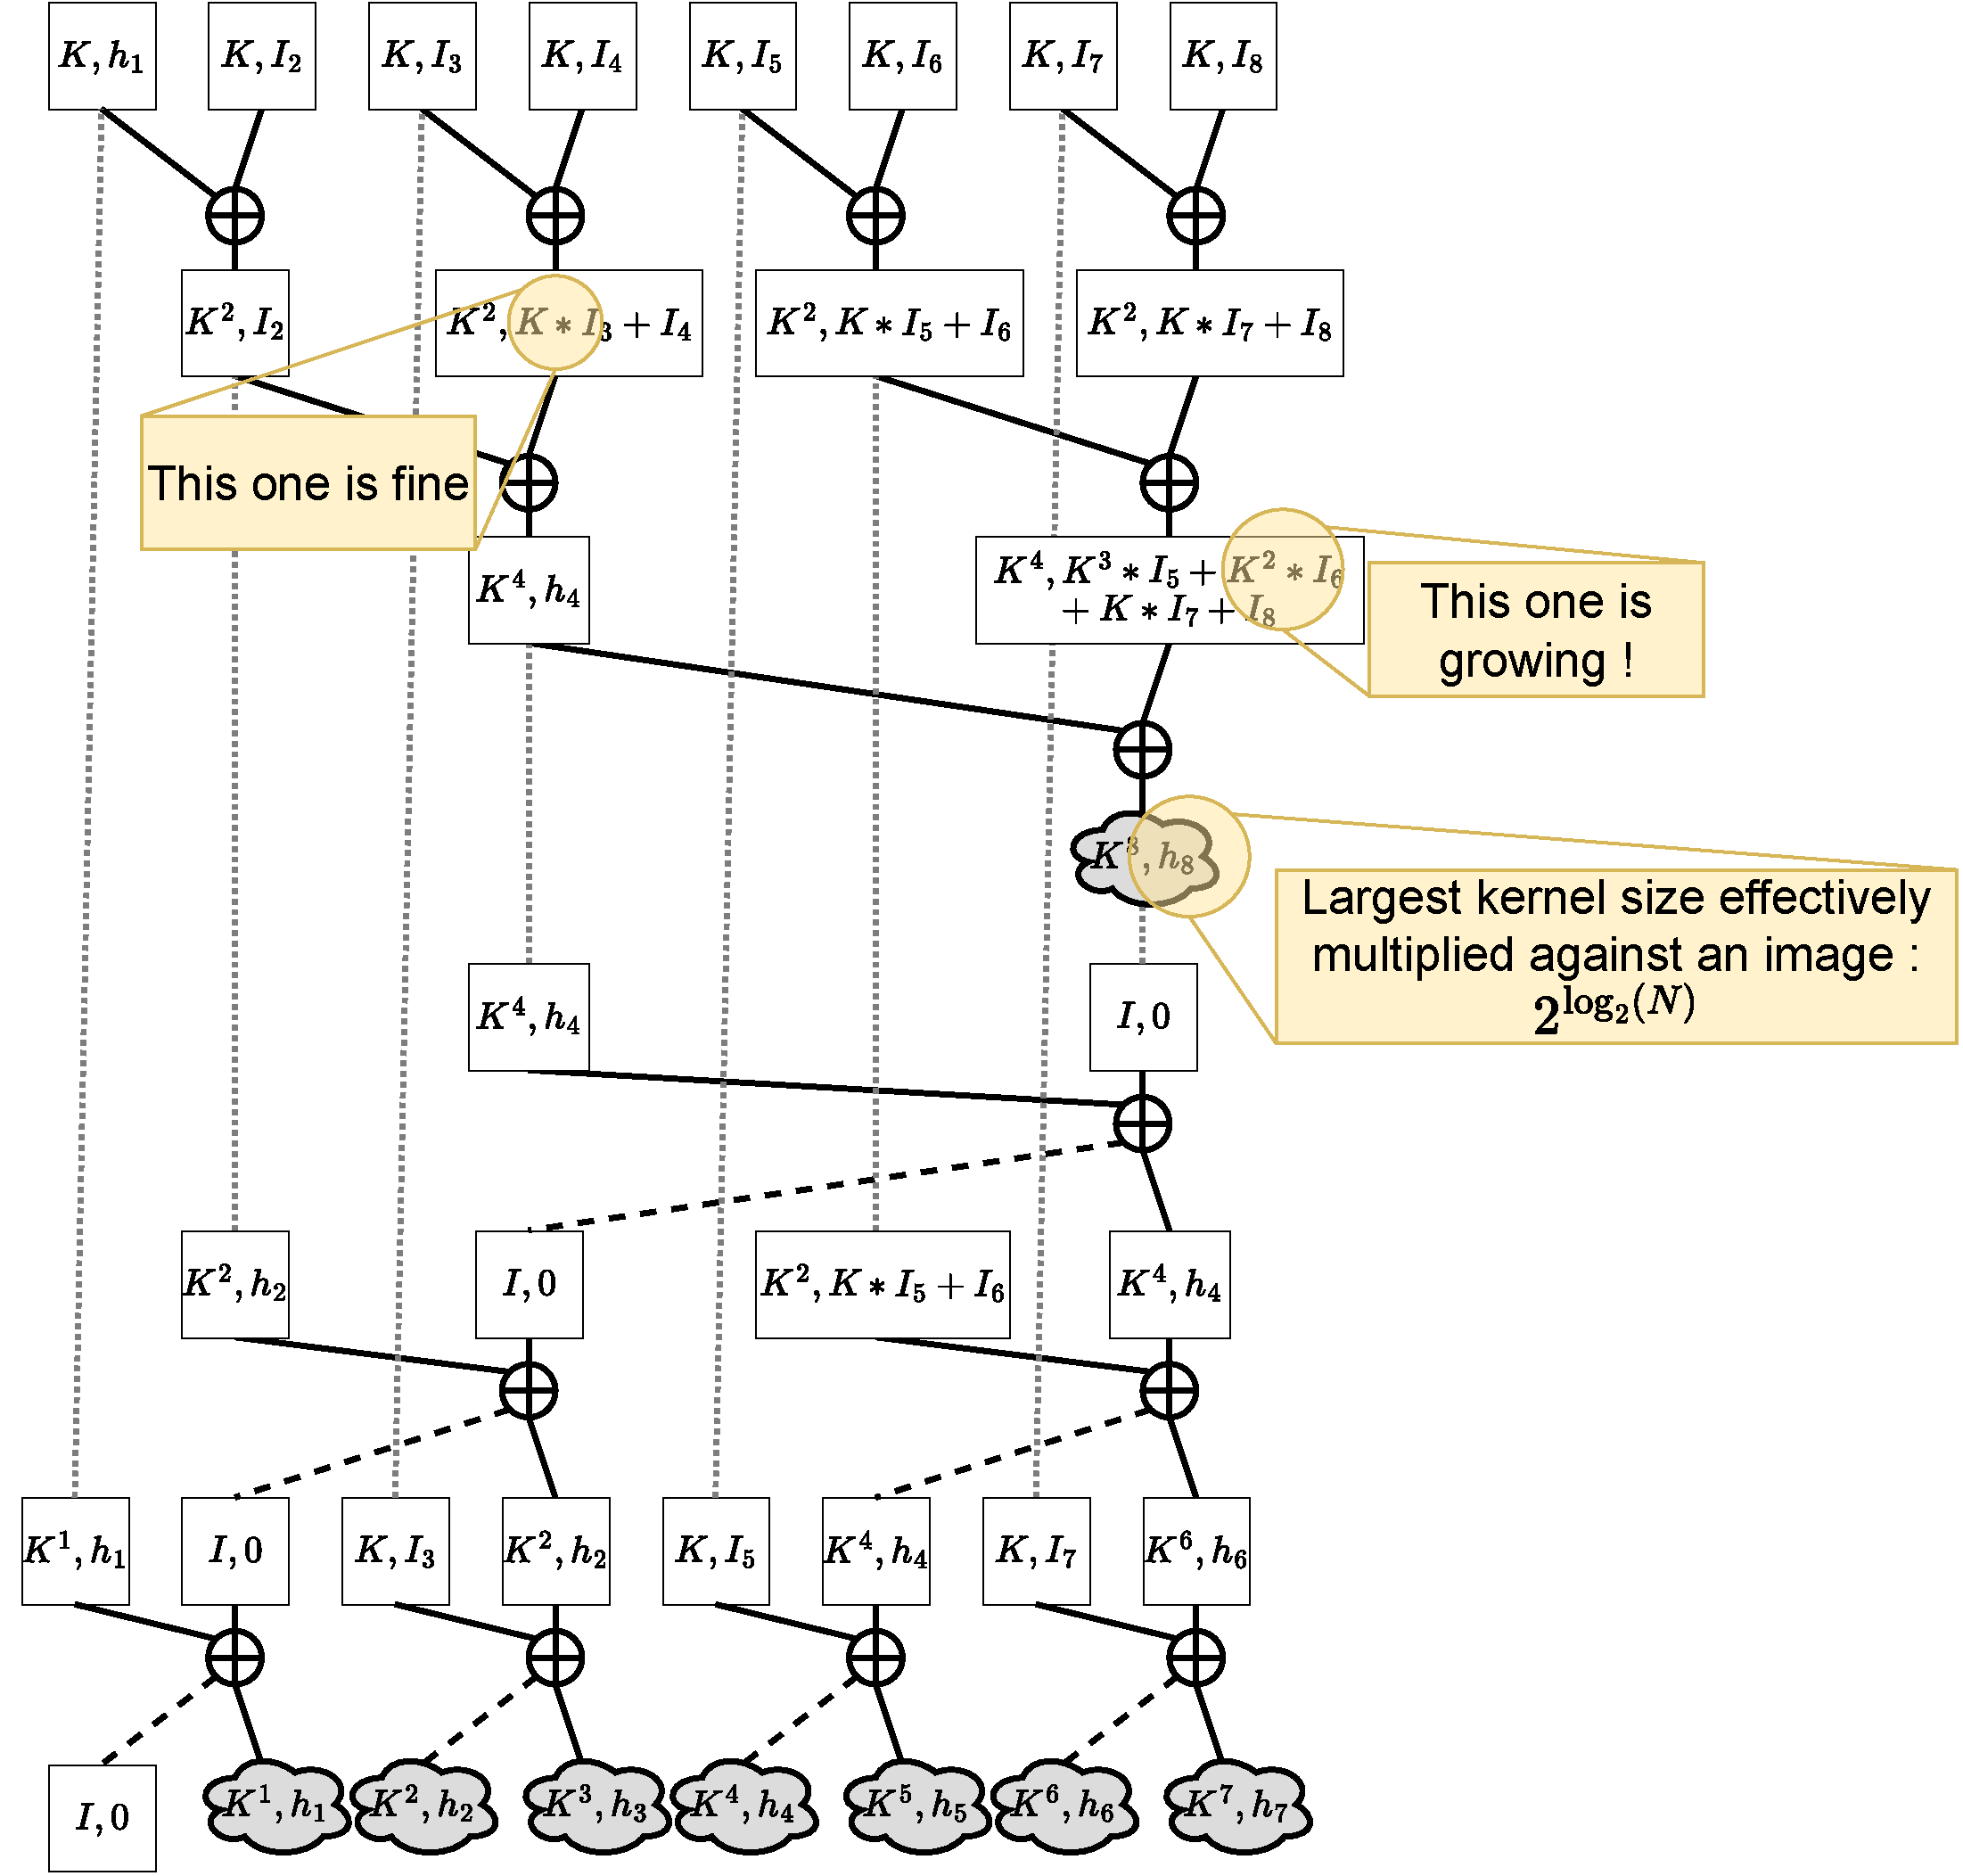
\includegraphics[height=0.3\textheight]{figures/scan_conv.pdf}
    \caption{Parallel scan applied to the monoid structure defined for spatial convolution SSM. Highlighted is the core of the issue : growing kernels lead to a bottleneck where a single operation has $O(T^2)$ complexity.}
    \label{fig:parallel_scan_conv_spatial}
\end{figure}

Moreover, as mentioned in the main text, the discretization step of the SSM leads to kernels with full spatial support, meaning that the initialization of the scan is $(a_t)_{t\in I} = ((\overline{\Kmat}_t, x_t))_{t\in I}$ with $\overline{\Kmat}_t$ of size $h \!\times\! w$. Thus, even the first step of the scan is intractable.

\subsection{Spectral ConvSSM Complexity}
\label{app:Spectral_ConvSSM_complexity}

To dispell the curse of growing kernels we move to the spectral domain and the ConvSSM formulation of \Cref{eq:convssm}. In this domain, our monoid becomes:
\begin{align}
\label{eq:M_SSM_spectral}
    &\mathcal{M}^{\mathrm{Conv}_2}\coloneqq \left\{ a = (\Lmat_c, x)\,\middle|\,\exists (\Kmat, x')\in \mathcal{M}^{\mathrm{Conv}_1},\Bigl\{
\begin{aligned}
    &\Lmat_c = P^{-1} \mathrm{Circ}(\Kmat_{\mathrm{padded}}) P \in \C^{hwc \times hwc}\\
    &x = P^{-1} x' \in \C^{h w c}
\end{aligned}
\Bigr.\right\}\\
\label{eq:+_SSM_spectral}
    &(\Lmat^a_c, x_a) \oplus^{\mathrm{Conv}_2} (\Lmat^b_c, x_b)\coloneqq (\Lmat^b_c \odot \Lmat^a_c, \Lmat^b_c \cdot x_a + x_b)\\
\label{eq:0_SSM_spectral}
    &e\coloneqq(I, 0)
\end{align}
\noindent with $\odot$ the element-wise matrix multiplication and $\cdot$ the element-wise matrix-vector multiplication. With this operator, the kernel grows no more, the cost is again a constant of time and depth, depending only on $h$, $w$ and $c$. We are thus back to a time complexity for the parallel scan of $O(\log T)$.

\begin{proposition}[Spectral ConvSSM Complexity]
    Let $(\mathcal{M}, +) \coloneqq (\mathcal{M}^{\mathrm{Conv}_2}, \oplus^{\mathrm{Conv}_2})$ be the monoid defined by \Cref{eq:M_SSM_spectral,eq:+_SSM_spectral,eq:0_SSM_spectral}. Let $(a_i)_{i\in I}\in (\mathcal{M}^{\mathrm{Conv}_2})^I$.

\begin{align}
    W&= O(T)\\
    T_\infty&= O(\log_2T)
\end{align}
\end{proposition}

\begin{proof}
The proof of \Cref{prop:scan_integer_complexity} applies with the only difference that now, each $\oplus^{\mathrm{Conv}_2}$ operation has complexity $h w c^3$ for the kernel-kernel multiplication on the left, $h w c^2$ for the kernel-image multiplication and $h w c$ for the image addition on the right. This gives :

\begin{align}
\label{eq:W_spectral}
    W&= O(T \times h w c^3)\\
\label{eq:T_spectral}
    T_\infty&= O(\log_2T \times h w c^3)
\end{align}
\end{proof}

\subsection{Taking down the constant factors}
\label{app:constant_factors}

Now that we have solved the main issue of complexity explosion with time, we tackle the problem of the constant factor. As mentioned in \Cref{prop:SSM_complexity}, as is, the work complexity is $O(T)$ with a constant that is $O(d^3)$ due to matrix multiplications.
%
The diagonal SSM (\Cref{eq:ssm:diagonal}) reduces this constant from $O(d^3)$ to $O(d)$. The complexity gain comes from the change of basis being absorbed outside of the recurrence such that the recurrence can operate on diagonalized matrices.

In the case of the Spectral SSM (\Cref{eq:ssm:spectral}), the $O(c^3)$ is even more prohibitive as it is repeated over each pixel position, with the total constant being $O(hwc^3)$ in the spectral domain (\Cref{eq:W_spectral,eq:T_spectral}). Hence the diagonal spectral SSM (\Cref{eq:ssm:diagonal_spectral}), which reduces the constant to $O(hwc)$. Our ConvSSM formulation (\Cref{eq:convssm}) exploits this diagonal spectral SSM and couples it with convolutional input and output transforms in order to make the whole model tractable.

\end{document}
